\documentclass{article}
\usepackage{graphicx}
\usepackage{float}
\usepackage[margin=0.5in]{geometry}
\usepackage{caption}
\usepackage{subcaption}

\usepackage{Sweave}
\begin{document}
\Sconcordance{concordance:HW2-latex.tex:HW2-latex.Rnw:%
1 7 1 1 0 202 1}


\title{STA511 Homework \#2}
\date{October 14, 2015}
\author{Abbas Rizvi}
\maketitle

\begin{enumerate}

\item No work required for question 1

\item Newton Raphson algorithm was implemented from a beta distribution for 100 observations. The stopping rule was $| x_i - x_{i-1}|$. Using {\tt{set.seed(333)}}, the average number of iterations was 3.5, and the accepted observations can be seen in Figure 1.  

\begin{figure}[htpb]
\centering
\caption{Histogram of Accepted Observations From Beta Distribution using Newton-Raphson method.}
\centering
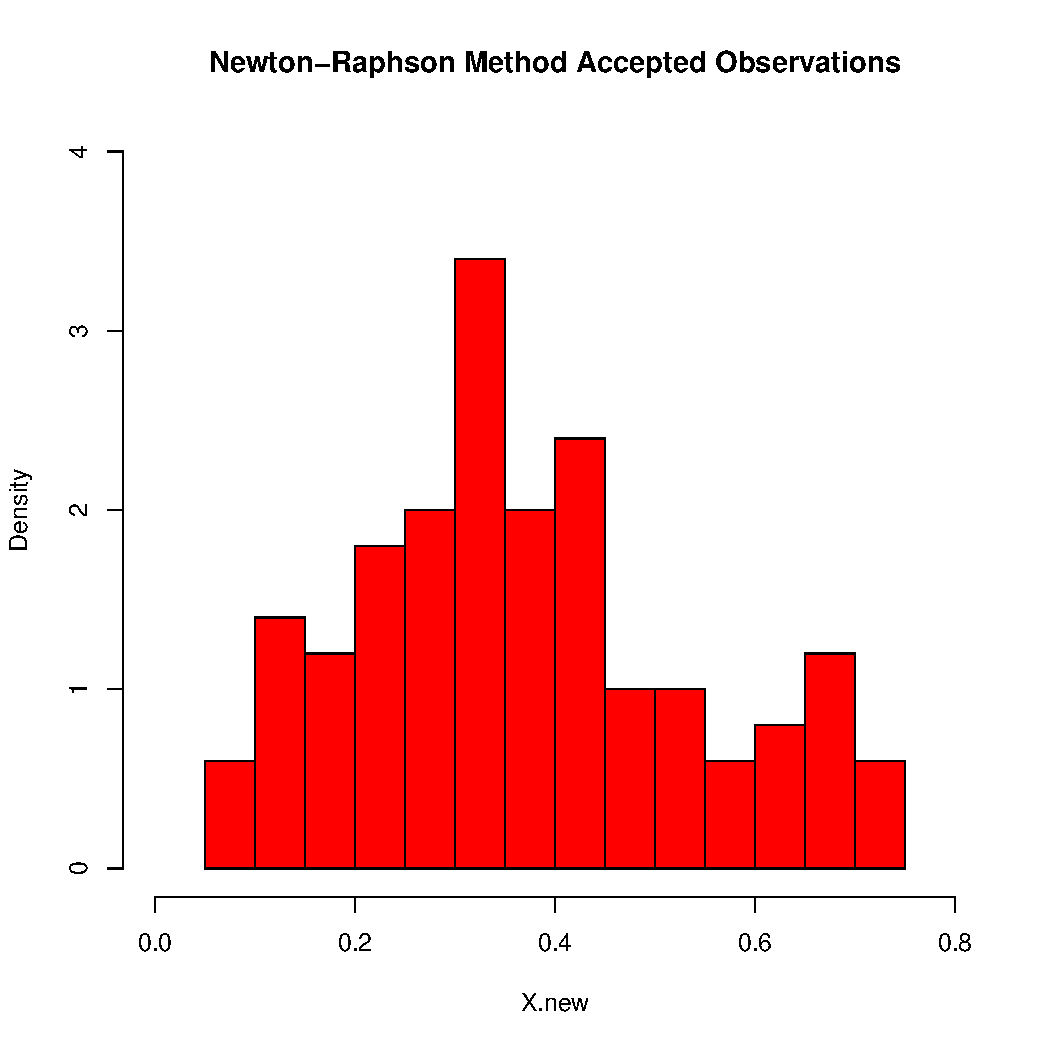
\includegraphics[scale=0.3]{/Users/aarizvi/Desktop/ROSWELL_PHD/STA511_StatisticalComputing/HW2/hw2-q2.pdf}
\end{figure}
The R code for Question 2 can be seen below:\\
\begin{verbatim}
rm(list=ls())
set.seed(333)
nsims <- 100
iterations <- c()
X.new <- c()
random.dist <- runif(1000)
for(i in 1:nsims){
        U <- random.dist[i]
        alpha <- 3
        beta <- 5
        x.old <- 0.5
        N <- 10 #random number that is bigger than 1 so 'j' in the while loop keepings resetting
        j <- 1
        while(j <= N){
                x.new <- x.old - ((pbeta(x.old, alpha, beta) - U)/dbeta(x.old, alpha, beta))
                j <- j + 1
                if(abs(x.new - x.old) < 0.05) {
                        break
                }
                x.old <- x.new
        }
        X.new[i] <- x.new
        print(X.new)
        iterations[i] <- j
}

mean(iterations)

pdf("hw2-q2.pdf")
hist(X.new, xlim=c(0,0.8), ylim=c(0,4), probability=TRUE, breaks=20, col="red",
     main="Newton-Raphson Method Accepted Observations")
dev.off()
\end{verbatim}
\item The Chi-square ($\chi^2$) and Kolmogorov-Smirnov (KS) tests were compared for type I error (part a) and power (part b).

\begin{enumerate}
\item Random uniform numbers between 0 and 1 were generated using the {\tt{runif}} command in R, with sample sizes of n = 10, 25, 50, 100. This was simulated 500 times and the p-values $< 0.05$ were reported in Table 1. The results can be interpreted such that as sample size increases towards n=50, the the type I error increases for the $\chi^2$ increases to about 5\%. As the sample size increases past n=50, the type I error begins to decrease. The KS type I errors that fell under the p-value $< 0.05$ criteria, were always around 0.05 no matter how large the sample size increased. This indicates that the KS value may be more appropriate for small and larger sample sizes. 

% latex table generated in R 3.1.2 by xtable 1.7-4 package
% Wed Oct 14 12:30:05 2015
\begin{table}[ht]
\centering
\caption{Type I Error was compared between Chi-squared and Kolmogorov-Smirnoff Tests. The values shown are the frequency of acceped type I error p-values (p $<$ 0.05) relative to total number of simulations}
\begin{tabular}{rrr}
  \hline
 & Chi-square Test & Kolmogorov-Smirnoff Test \\
  \hline
n = 10 & 0.024 & 0.050 \\ 
  n = 25 & 0.034 & 0.048 \\ 
  n = 50 & 0.046 & 0.046 \\ 
  n = 100 & 0.030 & 0.054 \\ 
   \hline
\end{tabular}
\end{table}

The code for question 3a:

\begin{verbatim}
rm(list=ls())
set.seed(333)
sample.size <- c(10, 25, 50, 100) #n = 10, 25, 50, 100
nsims <- 500

mat <- matrix(c(1:2*length(sample.size)),ncol=2, nrow=length(sample.size))

for (i in 1:length(sample.size)){
        ks.results <- list()
        chisq.results <- list()
        for (j in 1:nsims){
                r <- runif(sample.size[i])
                ks.results[j] <- ks.test(r, "punif", 0, 1)$p.value 
                #punif because you need to compare cdf
                r.counts <- hist(r, breaks=10, plot=FALSE)$counts 
                #using 10 bins for making counts
                chisq.results[j] <- chisq.test(r.counts)$p.value
        }
        chi.final <- list(sum(chisq.results <= 0.05))
        ks.final <- list(sum(ks.results <= 0.05))
        mat[i,1:2] <- do.call("cbind",c(chi.final,ks.final))
}
colnames(mat) <- c("Chi-square Test", "Kolmogorov-Smirnoff Test")
rownames(mat) <- paste("n", sample.size, sep=" = ")
\end{verbatim}

\item The power was compared between ${\chi^2}$ and KS tests. The power increased as sample size increased for ${\chi^2}$. As shown in Table 2, the power was again towards its maximum for any sample size, similar to the type I error result. This indicates that the KS test has more power when computing random beta distributions. This may be because {\tt{rbeta}} is NOT a good random number generator. 

\begin{table}[ht]
\centering
\caption{Chi-square and KS test compared for Power. The accepted values presented are frequencies relative to total number of simulations.}
\begin{tabular}{rrr}
  \hline
 & Chi-square Test & Kolmogorov-Smirnoff Test \\ 
  \hline
n = 10 & 0.01 & 1.00 \\ 
  n = 25 & 0.14 & 1.00 \\ 
  n = 50 & 0.57 & 1.00 \\ 
  n = 100 & 0.98 & 1.00 \\ 
   \hline
\end{tabular}
\end{table}
The code for question 3b is:
\begin{verbatim}
rm(list=ls())
set.seed(333)
sample.size <- c(10, 25, 50, 100)
shape1 <- 3
shape2 <- 5
nsims <- 500

mat <- matrix(c(1:2*length(sample.size)),ncol=2, nrow=length(sample.size))

for (i in 1:length(sample.size)){
        ks.results <- list()
        chisq.results <- list()
        for (j in 1:nsims){
                #rbeta with shape1=3, shape2=5
                r <- rbeta(sample.size[i], shape1, shape2) 
                #pbeta because you need to compare cdf
                ks.results[j] <- ks.test(r, "pbeta", 0, 1)$p.value
                #using 10 bins for making counts
                r.counts <- hist(r, breaks=10, plot=FALSE)$counts 
                chisq.results[j] <- chisq.test(r.counts)$p.value
        }
        chi.final <- list(sum(chisq.results <= 0.05))
        ks.final <- list(sum(ks.results <= 0.05))
        mat[i,1:2] <- do.call("cbind",c(chi.final,ks.final))
}
colnames(mat) <- c("Chi-square Test", "Kolmogorov-Smirnoff Test")
rownames(mat) <- paste("n", sample.size, sep=" = ")
\end{verbatim}

\end{enumerate}

\pagebreak

\item Simulation conducted to compare Type I error for Chi-squared test for a random number generator 0 to 1. The sample sizes used are n = 10, 25, 50, 100, 500. The bins used were bins = 10, 25, 50, 100, 500. The results of these simulations are reported in Table 3.  At a low sample sizes (n=10), as the number of bins increased, the more p-values that fall under the specified criteria (p $<$ 0.05) increase in frequency. However, as sample size increases, the trend appears to be less clear, showing a more uniform distribution of accepted p-values. Next time in order to help me interpret these results better I will plot the results in histograms as well for visualization, but unfortunately due to time constraints, I was unable to do this.
% latex table generated in R 3.1.2 by xtable 1.7-4 package
% Wed Oct 14 12:09:01 2015
\begin{table}[ht]
\centering
\caption{Simulation conducted to compare Type I error for Chi-squared test for a random number generator 0 to 1. The accepted values presented are frequencies relative to total number of simulations.}
\begin{tabular}{rrrrrr}
  \hline
 & n = 10 & n = 25 & n = 50 & n = 100 & n = 500 \\ 
  \hline
bin = 10 & 0.024 & 0.026 & 0.040 & 0.038 & 0.052 \\ 
  bin = 25 & 0.034 & 0.040 & 0.034 & 0.054 & 0.066 \\ 
  bin = 50 & 0.046 & 0.036 & 0.042 & 0.040 & 0.074 \\ 
  bin = 100 & 0.052 & 0.032 & 0.026 & 0.064 & 0.048 \\ 
  bin = 500 & 0.084 & 0.058 & 0.048 & 0.060 & 0.056 \\ 
   \hline
\end{tabular}
\end{table}

Here is the code for question 4:
\begin{verbatim}
rm(list=ls())
set.seed(333)
sample.size <- c(10,25,50,100,500)
bins <- c(10,25,50,100,500)
mat <- matrix(c(length(sample.size)*length(bins)),ncol=length(sample.size), nrow=length(bins))
nsims <- 500

for (i in 1:length(sample.size)){
        for (p in 1:length(bins)){
                chisq.results <- NULL             
                for (j in 1:nsims){
                        r <- round(runif(sample.size[i]),3)
                        r.counts <- hist(r, breaks=bins[p], plot=FALSE)$counts 
                        chisq.results[j] <- chisq.test(r.counts)$p.value
                }
                chi.final <- sum(chisq.results <= 0.05)
                mat[p,i] <- chi.final
        }
}
rownames(mat) <- paste("bin", bins, sep = " = ")
colnames(mat) <- paste("n", sample.size, sep = " = ")
print(mat)
\end{verbatim}
\end{enumerate}
\end{document}
